\xchapter{Estudo Experimental}{}
\label{estudo-experimental}

Este capítulo apresenta o processo de avaliação utilizado para medir a precisão do
sistema de identificação de momentos oportunos e inoportunos proposto. As seções deste
capítulo estão organizadas da seguinte forma: A Seção \ref{metodologia} apresenta a metodologia
utilizada para avaliar o sistema proposto. A Seção \ref{metricas} discorre sobre as métricas
utilizadas na avaliação. A Seção \ref{resultados} apresenta os resultados do experimento de
avaliação.

\section{Metodologia}
\label{metodologia}

O desempenho da proposta foi avaliado a partir de um experimento executado durante
situações reais de direção em um percurso em algumas ruas da cidade de Salvador -
Bahia.

O smartphone escolhido para realizar o experimento foi um OnePlus One com as seguintes características
\cite{oneplusone}:

\begin{itemize}
  \item Sistema Operacional: Cyanogen OS 13.1.2 (Android Marshmallow 6.0.1);
  \item CPU: Quad-Core 2.5 GHz Qualcomm Snapdragon 801;
  \item Memória RAM: 3 GB;
  \item Capacidade de armazenamento: 64 GB.
\end{itemize}

Para a realização do experimento foi criado no aplicativo Meu Possante uma tela com 5 botões, que serviu
para a identificação manual de cada momento. A tela pode ser vista na Figura \ref{tela-experimento}.

\begin{figure}[h]
\centering
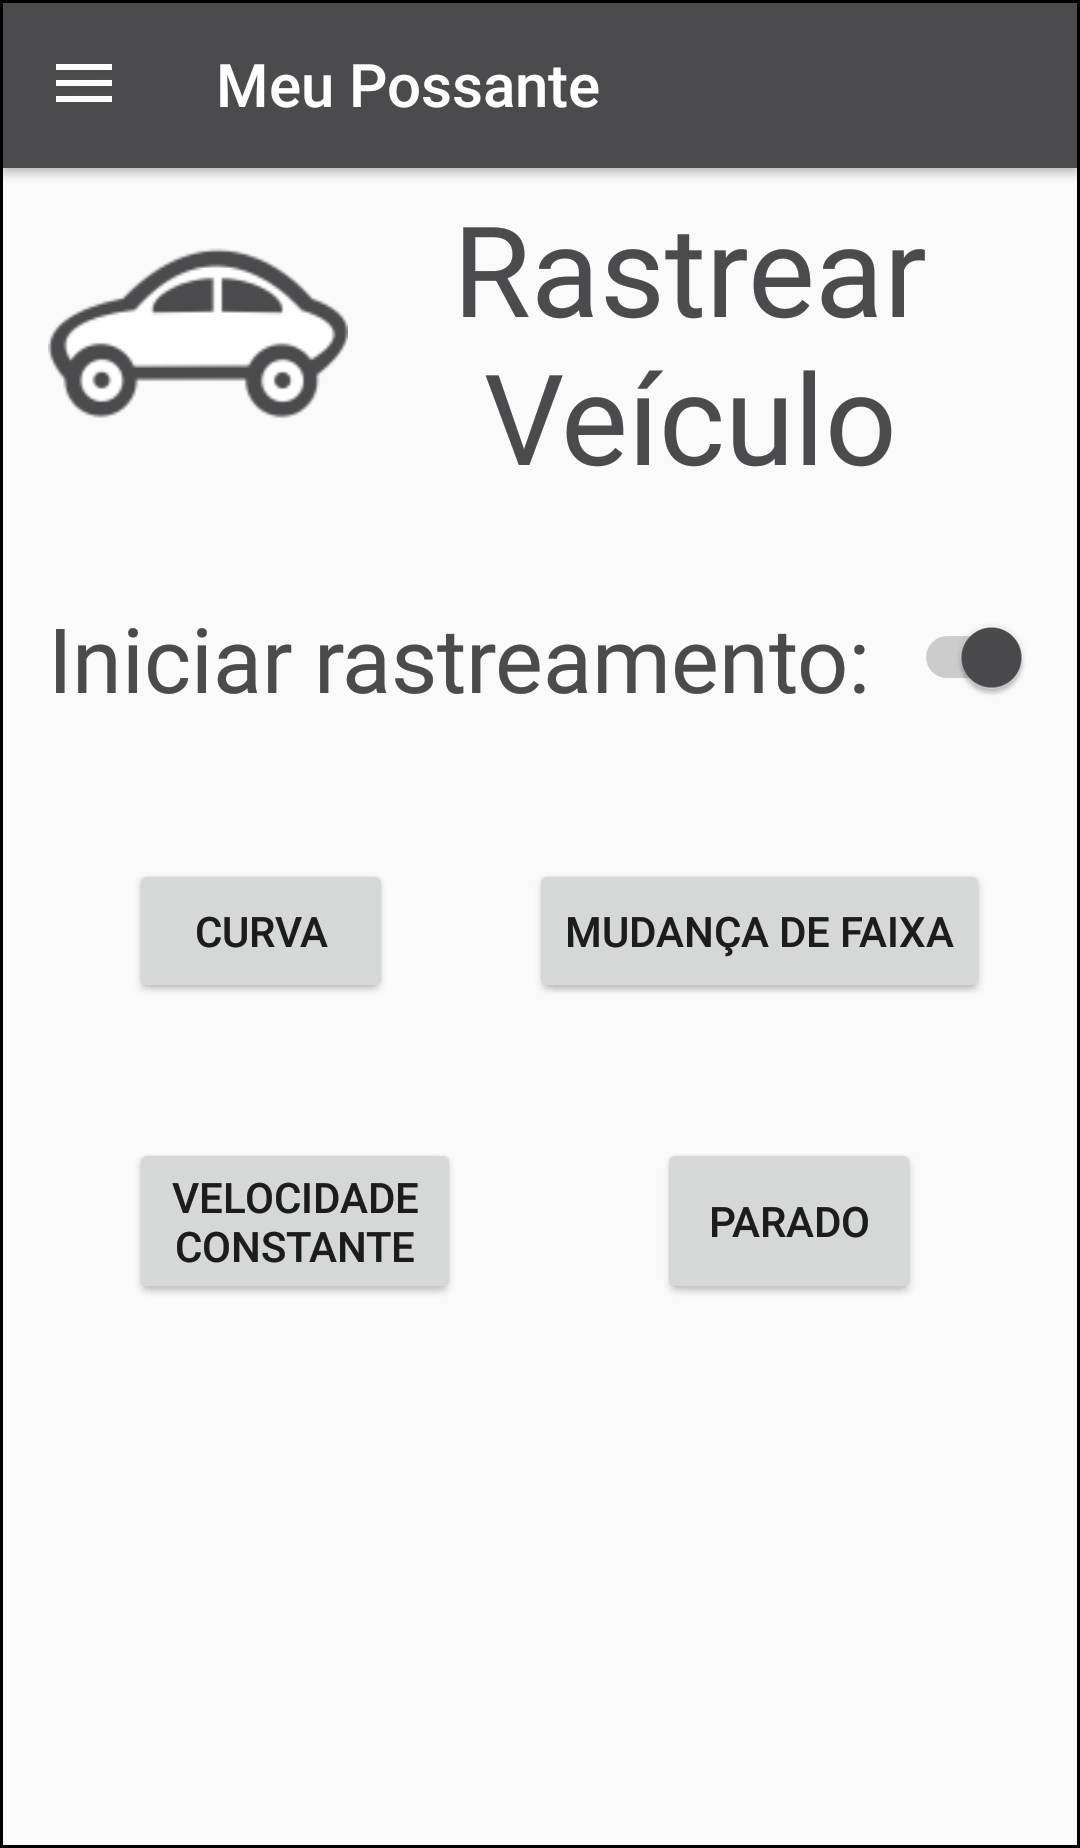
\includegraphics[width=0.3\textwidth]{images/tela-experimento.png}
\caption{Tela utilizada para auxiliar na identificação manual do momentos oportunos e inoportunos.}
\label{tela-experimento}
\end{figure}

Durante o experimento, ao passar por uma curva, por exemplo, o avaliador pressionava o botão
referente à curva, e informações do estado atual dos sensores eram guardadas em uma tabela no banco de dados.
Além disso, cada vez que o sistema detectava um momento oportuno ou inoportuno, um log sobre o
momento era guardado em outra tabela. Este log foi importante para a verificação dos falsos positivos.
O botão referente a nenhum momento foi importante para a detecção dos verdadeiros negativos utilizados
no cálculo da acurácia. A Seção \ref{metricas} discorre sobre isto.

O trajeto percorrido pelos participantes tinha 2,6 km de distância e era composto de 5 curvas à direita,
3 curvas à esquerda, 2 lugares com mudança de faixa e 3 semáforos. O experimento foi realizado com 3
voluntários, todos dirigindo seu próprio carro. O percurso está apresentado na Figura \ref{percurso} e os
indivíduos participantes do experimento estão listados na tabela \ref{participantes}.

\begin{figure}[H]
\centering
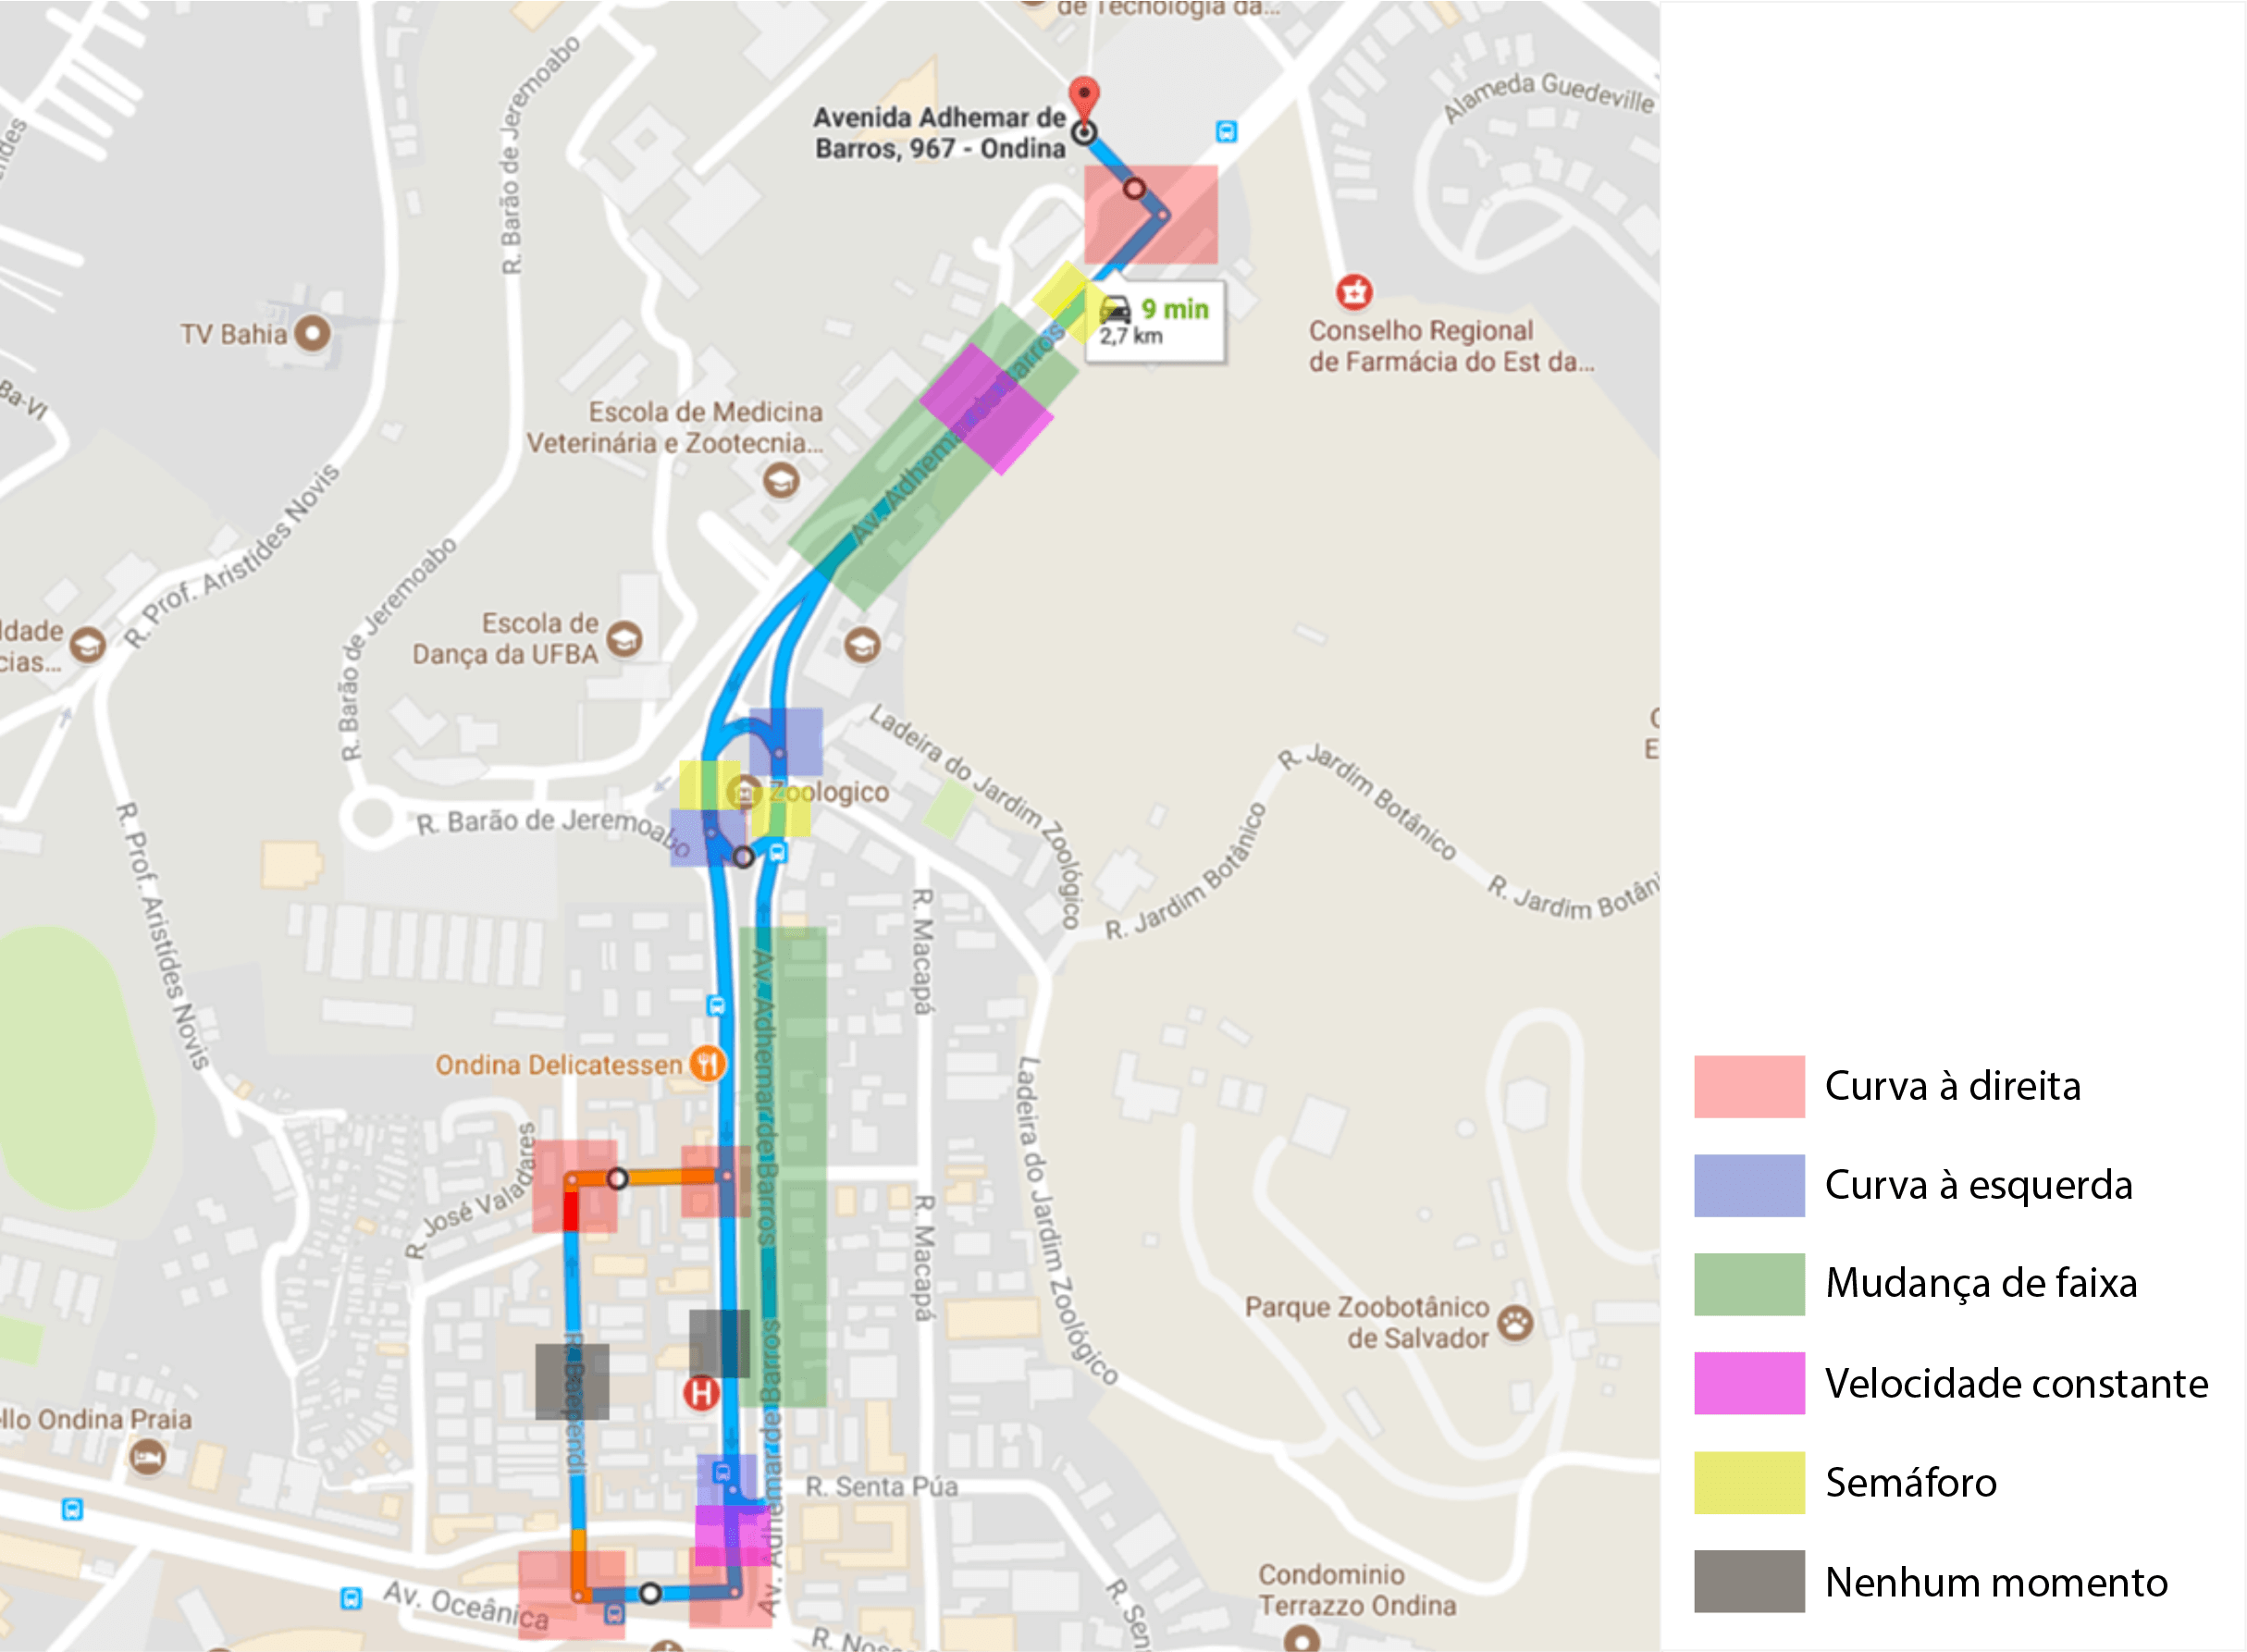
\includegraphics[width=0.63\textwidth]{images/percurso.png}
\caption{Percurso realizado no experimento de avaliação.}
\label{percurso}
\end{figure}

\begin{table}[h]
\centering
\caption{Indivíduos participantes do experimento}
\label{participantes}
\begin{tabular}{|c|c|c|c|}
\hline
\textbf{Indivíduo} & \textbf{Idade} & \textbf{Sexo} & \textbf{Carro utilizado} \\ \hline
Indivíduo 1        & 30             & Masculino     & Nissan Sentra            \\ \hline
Indivíduo 2        & 28             & Masculino     & Toyota Etios             \\ \hline
Indivíduo 3        & 24             & Feminino      & Chevrolet Prisma         \\ \hline
\end{tabular}
\end{table}

Antes do início do experimento os participantes foram instruídos a dirigir por todo o trajeto com
velocidade constante de 25 km/h. Como o trajeto era pré-definido, todos os participantes executaram
as mesmas tarefas na mesma ordem. Esta instruções, juntamente com os demais elementos do trajeto,
permitiram que todos os momentos, oportunos e inoportunos, fossem avaliados durante o experimento.

\section{Métricas de avaliação}
\label{metricas}

Para analisar o desempenho do sistema foi utilizada a métrica de acurácia. A acurácia é expressa pela
fórmula \ref{formula-acuracia}.

\begin{equation}
  Acur\acute{a}cia = \frac{TP + TN}{TP + FP + TN + FN}
\label{formula-acuracia}
\end{equation}

As variáveis da fórmula são as seguintes:

\begin{itemize}
  \item \textbf{TP:} True Positive (Verdadeiro Positivo em inglês). No experimento é dada pelo número de
  momentos identificados corretamente.
  \item \textbf{FP:} False Positive (Falso Positivo em inglês). No âmbito do experimento representa os
  momentos identificados erroneamente, ou seja, um momento que o sistema identificou mas que não ocorreu
  realmente.
  \item \textbf{TN:} True Negative (Verdadeiro Negativo em inglês). Representa os momentos que não ocorreram
  e que não foram identificados pelo sistema.
  \item \textbf{FN:} False Negative (Falso Negativo em inglês). Representa os momentos que ocorreram mas
  que não foram reconhecidos pelo sistema.
\end{itemize}

\section{Resultados}
\label{resultados}

Durante o experimento descrito na Seção \ref{metodologia} foram coletadas a seguinte quantidade de amostras para cada momento:

\begin{itemize}
  \item Curva: 98 amostras;
  \item Mudança de faixa: 29 amostras;
  \item Veículo parado: 27 amostras;
  \item Velocidade constante: 43 amostras;
  \item Nenhum momento: 26 amostras.
\end{itemize}

A tabela \ref{tabela-resultados} mostra os resultados do experimento de identificação de momentos oportunos e inoportunos.

\begin{table}[h]
\centering
\caption{Resultados do experimento de identificação dos momentos}
\label{tabela-resultados}
\resizebox{\textwidth}{!}{
\begin{tabular}{|c|c|c|c|c|}
\hline
\multicolumn{1}{|l|}{} & \multicolumn{2}{c|}{\textbf{Momentos Inoportunos}} & \multicolumn{2}{c|}{\textbf{Momentos Oportunos}}        \\ \hline
\textbf{Resultados}    & \textbf{Curva}     & \textbf{Mudança de Faixa}     & \textbf{Veículo Parado} & \textbf{Velocidade Constante} \\ \hline
Verdadeiros Positivos  & 94,89\%            & 75,86\%                       & 100\%                   & 72,1\%                        \\ \hline
Falsos Positivos       & 7,7\%              & 7,7\%                         & 0\%                     & 26,92\%                       \\ \hline
Verdadeiros Negativos  & 92,3\%             & 92,3\%                        & 100\%                   & 73,07\%                       \\ \hline
Falsos Negativos       & 5,11\%             & 24,13\%                       & 0\%                     & 27,9\%                        \\ \hline
Acurácia               & 95,35\%            & 84,08\%                       & 100\%                   & 72,58\%                       \\ \hline
\end{tabular}
}
\end{table}

O sistema apresentou resultados satisfatórios na detecção de curvas e do veículo parado, obtendo uma acurácia de 95,35\% e 100\% respectivamente. A
acurácia da detecção de mudança de faixa foi de 84,08\% e foi influenciada pela baixa velocidade do percurso, já que a velocidade angular medida pelo
giroscópio é influenciada pela velocidade do veículo. Por fim, a acurácia da identificação de velocidade constante foi de 72,58\% e pode ter sido
influenciada pela dificuldade do motorista em atender a orientação de manter a velocidade constante do veículo devido a imprevistos, como via congestionada,
outros carros parando bruscamente e pessoas atravessando a rua fora do semáforo. Mais experimentos são necessários para validar esta hipótese.

A acurácia total do sistema foi de 88\%. Alguns trabalhos relacionados podem trazer uma luz sobre este número. O classificador proposto por
\citeonline{kim2015sensors} para identificar momentos oportunos e inoportunos, obteve uma acurácia de 94\%, entretanto, este utilizava 7
sensores para a detecção, muitos não facilmente encontrados, enquanto que o presente trabalho utiliza apenas 2 sensores presentes na maioria dos
smartphones atuais. O sistema construído por \citeonline{johnson2011driving} para identificar comportamentos agressivos no trânsito obteve
97\% de acurácia utilizando 3 sensores, sendo um deles a câmera, que exige a montagem em uma posição específica no veículo e que pode ser afetada
pela iluminação e condição temporais.
